The retained full-duration study contains 80 verified core comparisons out of 80, 10 no-fault controls out of ten, and 20 background ablation runs out of twenty. Every declared trial and retry remains in the manifest. The corresponding raw outcomes and frozen source are available in checksum-verified bundles.

The replacement comparison uses 32 and 64 requests/s per cohort after two independent full-length no-fault qualifications at each rate. Admission required per-stream 99 percent Wilson upper screening bounds below half the SLO bad fractions, no dropped iterations or pod drift, and explicit CPU headroom. Earlier 48/112 requests/s studies were superseded after recurrent invalid high-load execution; their completed trials are not pooled into this comparison and their failed attempts remain archived. Independent cost pilots at 48 requests/s were retained. This is a revised workload protocol, not confirmation that the earlier stalls have a single proven cause.

\begin{table*}[width=\textwidth,cols=6,pos=t]
\caption{Closed-loop minus comparator differences in usable-guard overshoot. Intervals use paired run-block bootstrap resampling; negative values favor closed-loop on this metric only.}\label{tbl:paired}
\small
\begin{tabular*}{\tblwidth}{@{\extracolsep{\fill}}lllrll@{}}
\toprule
Fault & Requests/s & SLO & Comparator & Mean difference & 95\% interval \\
\midrule
abort & 32 & availability & static & -4.60 & [-6.80, -2.60] \\
abort & 32 & availability & threshold & 0.00 & [0.00, 0.00] \\
abort & 32 & availability & open-loop & 0.00 & [0.00, 0.00] \\
abort & 32 & latency & static & -4.60 & [-6.80, -2.60] \\
abort & 32 & latency & threshold & 0.00 & [0.00, 0.00] \\
abort & 32 & latency & open-loop & 0.00 & [0.00, 0.00] \\
abort & 64 & availability & static & -21.60 & [-26.00, -17.20] \\
abort & 64 & availability & threshold & 0.00 & [0.00, 0.00] \\
abort & 64 & availability & open-loop & 0.00 & [0.00, 0.00] \\
abort & 64 & latency & static & -21.60 & [-26.00, -17.20] \\
abort & 64 & latency & threshold & 0.00 & [0.00, 0.00] \\
abort & 64 & latency & open-loop & 0.00 & [0.00, 0.00] \\
delay & 32 & availability & static & 0.00 & [0.00, 0.00] \\
delay & 32 & availability & threshold & 0.00 & [0.00, 0.00] \\
delay & 32 & availability & open-loop & 0.00 & [0.00, 0.00] \\
delay & 32 & latency & static & -9.20 & [-12.00, -6.20] \\
delay & 32 & latency & threshold & 0.40 & [0.00, 1.20] \\
delay & 32 & latency & open-loop & 0.40 & [0.00, 1.20] \\
delay & 64 & availability & static & 0.00 & [0.00, 0.00] \\
delay & 64 & availability & threshold & 0.00 & [0.00, 0.00] \\
delay & 64 & availability & open-loop & 0.00 & [0.00, 0.00] \\
delay & 64 & latency & static & -16.20 & [-24.40, -8.40] \\
delay & 64 & latency & threshold & 0.00 & [0.00, 0.00] \\
delay & 64 & latency & open-loop & 0.00 & [0.00, 0.00] \\
\bottomrule
\end{tabular*}
\end{table*}

Full-allocation overshoot, exposure differences, observed failures and empirical costs appear in the accompanying CSV tables. A guard-overshoot improvement alone does not establish a better safety/exposure trade-off. The intervals are descriptive, with only five blocks and no multiplicity adjustment. Any missing pair remains explicitly incomplete rather than disappearing from analysis.

\begin{figure*}
\centering
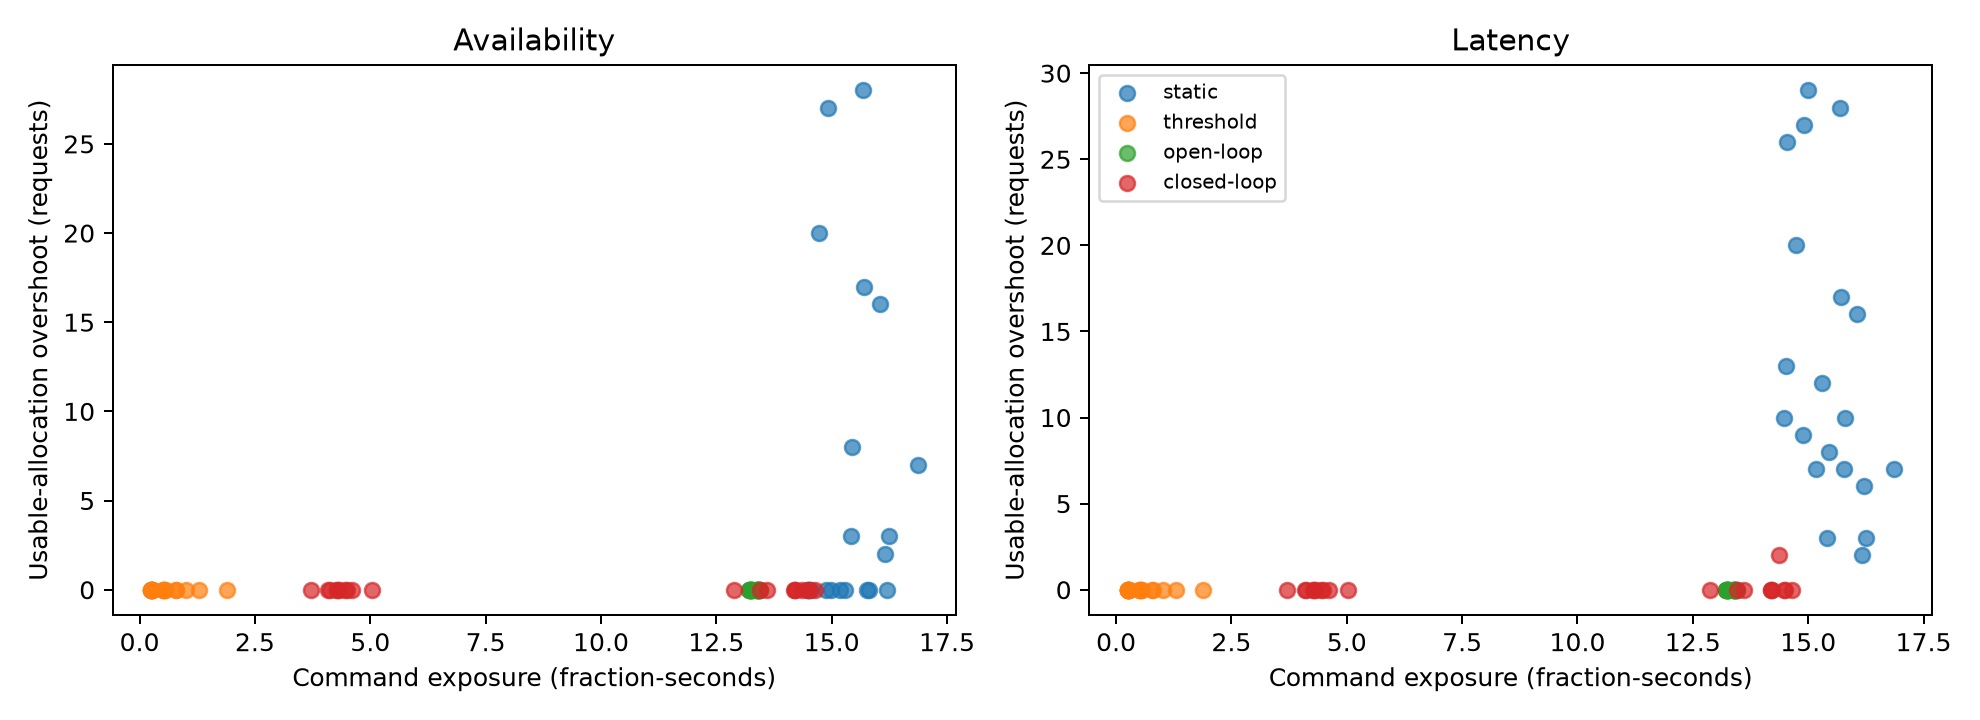
\includegraphics[width=.96\textwidth]{results/curated/study-comparison.png}
\caption{Every verified core run, showing exposure against overshoot of the usable allocation. Full-allocation overshoot is separately retained in the raw tables.}\label{fig:study}
\end{figure*}
\subsection{Controlled background attribution}\label{sec:background}
At 32 requests/s, availability point-estimate minus naive-total absolute error was -66.78 requests (95\% interval [-68.38, -64.97]). At 32 requests/s, latency point-estimate minus naive-total absolute error was -66.78 requests (95\% interval [-68.38, -64.97]). At 64 requests/s, availability point-estimate minus naive-total absolute error was -134.60 requests (95\% interval [-138.20, -130.99]). At 64 requests/s, latency point-estimate minus naive-total absolute error was -134.60 requests (95\% interval [-138.20, -130.99]). The reference subtracts tagged synthetic organic failures; incidental non-organic failures and shared-node interference remain possible.
